\documentclass[twoside,twocolumn]{article}

\usepackage{blindtext} % Package to generate dummy text throughout this template 
\usepackage{graphicx}
\usepackage[sc]{mathpazo} % Use the Palatino font
\usepackage[T1]{fontenc} % Use 8-bit encoding that has 256 glyphs
\linespread{1.05} % Line spacing - Palatino needs more space between lines
\usepackage{microtype} % Slightly tweak font spacing for aesthetics

\usepackage[english]{babel} % Language hyphenation and typographical rules

\usepackage[hmarginratio=1:1,top=32mm,columnsep=20pt]{geometry} % Document margins
\usepackage[hang, small,labelfont=bf,up,textfont=it,up]{caption} % Custom captions under/above floats in tables or figures
\usepackage{booktabs} % Horizontal rules in tables
\usepackage{graphicx}
\usepackage{lettrine} % The lettrine is the first enlarged letter at the beginning of the text

\usepackage{enumitem} % Customized lists
\setlist[itemize]{noitemsep} % Make itemize lists more compact

\usepackage{abstract} % Allows abstract customization
\renewcommand{\abstractnamefont}{\normalfont\bfseries} % Set the "Abstract" text to bold
\renewcommand{\abstracttextfont}{\normalfont\small\itshape} % Set the abstract itself to small italic text

\usepackage{titlesec} % Allows customization of titles
\renewcommand\thesection{\Roman{section}} % Roman numerals for the sections
\renewcommand\thesubsection{\roman{subsection}} % roman numerals for subsections
\titleformat{\section}[block]{\large\scshape\centering}{\thesection.}{1em}{} % Change the look of the section titles
\titleformat{\subsection}[block]{\large}{\thesubsection.}{1em}{} % Change the look of the section titles

\usepackage{fancyhdr} % Headers and footers
\pagestyle{fancy} % All pages have headers and footers
\fancyhead{} % Blank out the default header
\fancyfoot{} % Blank out the default footer
\fancyhead[C]{Comparativa de Gestores de Base de Datos No Relacionales $\bullet$ Octubre 2021 $\bullet$ } % Custom header text
\fancyfoot[RO,LE]{\thepage} % Custom footer text

\usepackage{titling} % Customizing the title section

\usepackage{hyperref} % For hyperlinks in the PDF

%----------------------------------------------------------------------------------------
%	TITLE SECTION
%----------------------------------------------------------------------------------------
\providecommand{\keywords}[1]{
  \small	
  \textbf{\textit{\quad \quad Keywords: }} #1}

\providecommand{\pclave}[1]{
  \small	
  \textbf{\textit{\quad \quad Palabras Clave: }} #1}

%Idiomas: \selectlanguage{english} \selectlanguage{spanish}

\begin{document}

\title{Trabajo Encargado N°1: Comparativa de Gestores de Base De Datos No Relacionales}

\begin{titlepage}
\begin{figure}[htb]
\begin{center}

\includegraphics[width=5cm]{imagenes/logo.png}
\end{center}
\end{figure}
\vspace*{-0.25in}
\begin{center}
\large{UNIVERSIDAD PRIVADA DE TACNA}\\
\vspace*{-0.025in}
INGENIERIA DE SISTEMAS  \\

\vspace*{0.5in}
\begin{large}
TITULO:\\
\end{large}

\vspace*{0.1in}
\begin{Large}
\textbf{Comparativa de Gestores de Base De Datos No Relacionales} \\
\end{Large}

\vspace*{0.3in}
\begin{Large}
\textbf{CURSO:} \\
\end{Large}

\vspace*{0.1in}
\begin{large}
Base de Datos II\\
\end{large}

\vspace*{0.3in}
\begin{Large}
\textbf{DOCENTE:} \\
\end{Large}

\vspace*{0.1in}
\begin{large}
 Ing. Patrick Cuadros Quiroga\\
\end{large}

\vspace*{0.2in}
\vspace*{0.1in}
\begin{large}

Integrantes: \\
\begin{flushleft}
Maldonado Cancapi, Carlos Alejandro\hfill(2018000660) \\
Huillca Aroni, Alfredo\hfill(2018060903)\\
Huallpa Huayachani, Alexander Junior\hfill(2018062497)\\
Anahua Huayhua, Jenny Karen\hfill(2018062150)\\
Condori Ramirez, Laura Soledad\hfill(2006028408)\\
Soto Rodriguez, Daniela Duanet\hfill(2015051384)\\

\end{flushleft}
\end{large}

\vspace*{0.1in}
\begin{large}
Tacna - Perú\\
2021
\end{large}
\end{center}
\end{titlepage}

\setlength{\droptitle}{-4\baselineskip} % Move the title up

\pretitle{\begin{center}\Huge\bfseries} % Article title formatting
\posttitle{\end{center}} % Article title closing formatting
\title{Comparativa de Gestores de Bases de Datos No Relacionales} % Article title

\date{\today} % Leave empty to omit a date                     
\renewcommand{\maketitlehookd}{%

}

%----------------------------------------------------------------------------------------



% Print the title
\maketitle

%----------------------------------------------------------------------------------------
%	ARTICLE CONTENTS
%----------------------------------------------------------------------------------------

\section{Resumen}

\lettrine[nindent=0em,lines=3]{E}n el presente las bases de datos están inmersas en casi cualquier tipo de proyecto, Las bases de datos relacionales han dominado el mundo de la gestión de datos desde la década de los 70, pero el nacimiento de Internet y su auge como plataforma de aplicaciones ha puesto a prueba el dominio de las soluciones relacionales.
El volumen de datos al que debe hacer frente una aplicación web ha crecido exponencialmente, así como el número de usuarios que utiliza las aplicaciones y servicios disponibles en Internet, y en consecuencia el volumen de transacciones y la demanda a la que se ven sometidas, ya que los usuarios esperan un tiempo de respuesta inmediato en sus interacciones online con el website.
Las bases de datos NoSQL empezaron su aparición gracias a Google y Amazon, ambos con las soluciones de bases de datos BigTables y Dynamo respectivamente.
Las bases de datos no relacionales están diseñadas para ejecutarse sobre clústeres, es decir que pueden tener muchas maquinas pequeñas (bajo costo) ejecutando instancias de estas bases de datos.




%------------------------------------------------

\section{Abstract}


At present, databases are immersed in almost any type of project. 
Relational databases have dominated the world of data management since the 1970s,
but the birth of the Internet and its rise as an application platform has put 
the domain of relational solutions to the test.The volume of data that a web
application must deal with has grown exponentially, as well as the number of 
users who use the applications and services available on the Internet, and 
consequently the volume of transactions and the demand to which they are subjected,
already that users expect an immediate response time in their online interactions
with the website.NoSQL databases began their appearance thanks to Google and 
Amazon, both with BigTables and Dynamo database solutions
respectively.Non-relational databases are designed to run on clusters, that is,
they can have many small machines (low cost) running instances of these databases




%------------------------------------------------
\section{Introduccion}

Son muchas las aplicaciones web que utilizan algún tipo de bases de 
datos para funcionar. Hasta ahora estábamos acostumbrados a utilizar 
bases de datos SQL como son MySQL, Oracle o MS SQL, pero desde hace ya 
algún tiempo han aparecido otras que reciben el nombre de NoSQL 
(Not only SQL – No sólo SQL) y que han llegado con la intención de hacer
 frente a las bases relacionales utilizadas por la mayoría de los usuarios.

\section{Desarrollo}

\subsection{¿Qué son las bases de datos NoSQL?}

Se puede decir que la aparición del término NoSQL aparece con 
la llegada de la web 2.0 ya que hasta ese momento sólo subían 
contenido a la red aquellas empresas que tenían un portal, pero 
con la llegada de aplicaciones como Facebook, Twitter o Youtube, 
cualquier usuario podía subir contenido, provocando así un crecimiento
exponencial de los datos. Es en este momento cuando empiezan a aparecer
los primeros problemas de la gestión de toda esa información almacenada
en bases de datos relacionales. En un principio, para solucionar estos
problemas de accesibilidad, las empresas optaron por utilizar un mayor
número de máquinas pero pronto se dieron cuenta de que esto no solucionaba 
el problema, además de ser una solución muy cara. La otra solución era la
creación de sistemas pensados para un uso específico que con el 
paso del tiempo han dado lugar a soluciones robustas, apareciendo 
así el movimiento NoSQL. Por lo tanto hablar de bases de datos NoSQL 
es hablar de estructuras que nos permiten almacenar información en aquellas
situaciones en las que las bases de datos relacionales generan ciertos 
problemas debido principalmente a problemas de escalabilidad y rendimiento
de las bases de datos relacionales donde se dan cita miles de usuarios 
concurrentes y con millones de consultas diarias. Además de lo comentado 
anteriormente, las bases de datos NoSQL son sistemas de almacenamiento de
información que no cumplen con el esquema entidad–relación. Tampoco utilizan
una estructura de datos en forma de tabla donde se van almacenando los
datos sino que para el almacenamiento hacen uso de otros formatos como 
clave–valor, mapeo de columnas o grafos.

\subsection{Ventajas de los sistemas NOSQL}
\begin{itemize}
    \item 	Esta forma de almacenar la información ofrece ciertas ventajas sobre los modelos relacionales. Entre las ventajas más significativas podemos destacar: 
    \item 	Se ejecutan en máquinas con pocos recursos: Estos sistemas, a diferencia de los sistemas basados en SQL, no requieren de apenas computación, por lo que se pueden montar en máquinas de un coste más reducido. 
    \item 	Escalabilidad horizontal: Para mejorar el rendimiento de estos sistemas simplemente se consigue añadiendo más nodos, con la única operación de indicar al sistema cuáles son los nodos que están disponibles. 
    \item 	Pueden manejar gran cantidad de datos: Esto es debido a que utiliza una estructura distribuida, en muchos casos mediante tablas Hash.
    \item 	No genera cuellos de botella: El principal problema de los sistemas SQL es que necesitan transcribir cada sentencia para poder ser ejecutada, y cada sentencia compleja requiere además de un nivel de ejecución aún más complejo, lo que constituye un punto de entrada en común, que ante muchas peticiones puede ralentizar el sistema.
    
\end{itemize}

   
\subsection{Principales diferencias con las bases de datos SQL}

Algunas de las diferencias más destacables que nos podemos encontrar entre los sistemas
 NoSQL y los sistemas SQL están: 
\begin{itemize}
    \item 	No utilizan SQL como lenguaje de consultas. La mayoría de las bases de datos NoSQL evitan utilizar este tipo de lenguaje o lo utilizan como un lenguaje de apoyo. Por poner algunos ejemplos, Cassandra utiliza el lenguaje CQL, MongoDB utiliza JSON o BigTable hace uso de GQL. 
    \item 	No utilizan estructuras fijas como tablas para el almacenamiento de los datos. Permiten hacer uso de otros tipos de modelos de almacenamiento de información como sistemas de clave–valor, objetos o grafos. 
    \item 	No suelen permitir operaciones JOIN. Al disponer de un volumen de datos tan extremadamente grande suele resultar deseable evitar los JOIN. Esto se debe a que, cuando la operación no es la búsqueda de una clave, la sobrecarga puede llegar a ser muy costosa. Las soluciones más directas consisten en desnormalizar los datos, o bien realizar el JOIN mediante software, en la capa de aplicación. 
    \item 	Arquitectura distribuida. Las bases de datos relacionales suelen estar centralizadas en una única máquina o bien en una estructura máster–esclavo, sin embargo en los casos NoSQL la información puede estar compartida en varias máquinas mediante mecanismos de tablas Hash distribuidas
     
    
\end{itemize}


\subsection{Tipos de bases de datos NoSQL}

Dependiendo de la forma en la que almacenen la información, nos podemos
encontrar varios tipos distintos de bases de datos NoSQL. Veamos los tipos 
más utilizados.


\subsubsection{Bases de datos clave – valor}

Son el modelo de base de datos NoSQL más popular, además de ser
 la más sencilla en cuanto a funcionalidad. En este tipo de sistema, 
 cada elemento está identificado por una llave única, lo que permite la
  recuperación de la información de forma muy rápida, información que 
  habitualmente está almacenada como un objeto binario (BLOB). Se caracterizan
   por ser muy eficientes tanto para las lecturas como para las escrituras.
    Algunos ejemplos de este tipo son Cassandra, BigTable o HBase.
    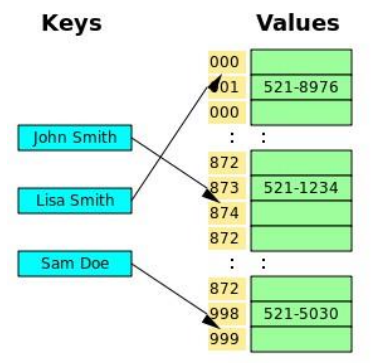
\includegraphics[width=7cm, height=7cm]{imagenes/img1.png}

\subsubsection{Bases de datos documentales}
Este tipo almacena la información como un documento,
generalmente utilizando para ello una estructura simple 
como JSON o XML y donde se utiliza una clave única para
cada registro. Este tipo de implementación permite, además
de realizar búsquedas por clave–valor, realizar consultas más
avanzadas sobre el contenido del documento. Son las bases de 
datos NoSQL más versátiles. Se pueden utilizar en gran cantidad 
de proyectos, incluyendo muchos que tradicionalmente funcionarían
sobre bases de datos relacionales. Algunos ejemplos de este tipo 
son MongoDB o CouchDB.
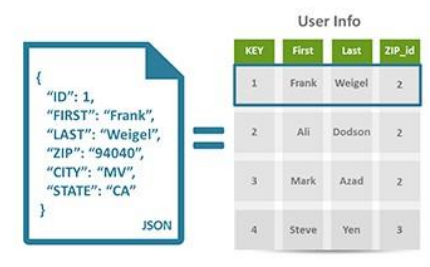
\includegraphics[width=7cm, height=7cm]{imagenes/img2.png}
\subsubsection{Bases de datos en grafo}
En este tipo de bases de datos, la información se 
representa como nodos de un grafo y sus relaciones 
con las aristas del mismo, de manera que se puede 
hacer uso de la teoría de grafos para recorrerla. Para 
sacar el máximo rendimiento a este tipo de bases de datos,
 su estructura debe estar totalmente normalizada, de forma que 
 cada tabla tenga una sola columna y cada relación dos. Este tipo 
 de bases de datos ofrece una navegación más eficiente entre relaciones
  que en un modelo relacional. Algunos ejemplos de este tipo son Neo4j, 
  InfoGrid o Virtuoso.
  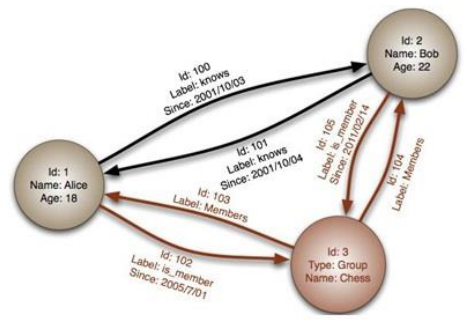
\includegraphics[width=7cm, height=7cm]{imagenes/img3.png}
\subsubsection{Bases de datos orientadas a objetos} 
En este tipo, la información se representa mediante objetos, de la misma 
forma que son representados en los lenguajes de programacion oriendata 
a objetos (POO) como ocurre en Java, C\# o Visual Basic .NET. Algunos ejemplos de este 
tipo de bases de datos son Zope, Gemstone o Db4o.
\subsection{Ejemplos de bases de datos NoSQL}  
Veamos a continuación algunas tipos de bases NoSQL más utilizadas actualmente. 
\subsubsection{Cassandra}
Se trata de una base de datos creada por Apache del tipo clave–valor. 
Dispone de un lenguaje propio para realizar consultas CQL (Cassandra Query Language). Cassandra es una aplicación Java por lo 
que puede correr en cualquier plataforma que cuente con la JVM.
\subsubsection{Redis}
Se trata de una base de datos creada por 
Salvatore Sanfilippo y Pieter Noordhuis y está 
apoyado por VMWare. Se trata de una base de datos del tipo clave–valor.
 Se puede imaginar como un array gigante en memoria para almacenar datos,
  datos que pueden ser cadenas, hashes, conjuntos de datos o listas. Tiene 
  la ventaja de que sus operaciones son atómicas y persistentes. Por ponerle 
  una pega, Redis no permite realizar consultas, sólo se puede insertar y
   obtener datos, además de las operaciones comunes sobre conjuntos 
   (diferencia, unión e inserción). Creado en ANSI C, por lo tanto es 
   compatible y funciona sin problemas en sistemas Unix, Linux y sus derivados,
    Solaris, OS/X sin 
embargo no existe soporte oficial para plataformas Windows.
\subsubsection{Mongodb}
Se trata de una base de datos creada por 10gen del tipo orientada a documentos, 
de esquema libre, es decir, que cada entrada puede tener un esquema de datos 
diferente que nada tenga que ver con el resto de registros almacenados. 
Es bastante rápido a la hora de ejecutar sus operaciones ya que está escrito
 en lenguaje C++. Para el almacenamiento de la información, utiliza un sistema
  propio de documento conocido con el nombre BSON, que es una evolución del 
  conocido JSON pero con la peculiaridad de que puede almacenar datos binarios.
   En poco tiempo, MongoDB se ha convertido en
 una de las bases de datos NoSQL favoritas por los desarrolladores.
\subsubsection{CouchDB}
Se trata de una base de datos creada por 10gen del tipo orientada a 
documentos, de esquema libre, es decir, que cada entrada puede tener 
un esquema de datos diferente que nada tenga que ver con el resto de 
registros almacenados. Es bastante rápido a la hora de ejecutar sus 
operaciones ya que está escrito en lenguaje C++. Para el almacenamiento 
de la información, utiliza un sistema propio de documento conocido con el
 nombre BSON, que es una evolución del conocido JSON pero con la peculiaridad
  de que puede almacenar datos binarios. En poco tiempo, MongoDB se ha convertido 
en una de las bases de datos NoSQL favoritas por los desarrolladores.

\subsection{Razones para usar NOSQL}
\begin{itemize}
    \item   Cuando el volumen de los datos crece muy rápidamente en momentos puntuales, pudiendo llegar a superar el Terabyte de información. 
    \item	Cuando la escalabilidad de la solución relacional no es viable tanto a nivel de costes como a nivel técnico. 
    \item	Cuando tenemos elevados picos de uso del sistema por parte de los usuarios en múltiples ocasiones. 
    \item	Cuando el esquema de la base de datos no es homogéneo, es decir, cuando en cada inserción de datos la información que se almacena puede tener campos distintos.
    
\end{itemize}
\subsection{Grandes compañías que utilizan este tipo de bases de datos}
Son muchas las grandes empresas que hacen uso de este tipo de bases de datos no relacionales, como: 
\begin{itemize}
    \item   Cassandra: Facebook, Twitter… 
    \item	HBase: Yahoo, Adobe… 
    \item	Redis: Flickr, Instagram, Github… 
    \item	Neo4j: Infojobs… 
    \item	MongoDB: FourSquare, SourceForge, CERN…
    
\end{itemize}

\subsection{Gestor de Base de datos-Mongodb}
Es el sistema de base de datos desarrollada en 10gen por Geir Magnusson 
y Dwight Merriman. Es una base de datos NoSQL orientada a documentos JSON,
está escrito en C++, 
aunque las consultas se hacen pasando objetos JSON como parámetro,
dado que los propios documentos se almacenan en BSON. Es la base de datos
NoSQL más utilizada en el mundo. Su nombre viene del término inglés “humongous” 
(colosal) y puede ser definida como una base de datos documental sin esquema, 
escalable y de alto rendimiento. Al ser un proyecto de código abierto, sus binarios
están disponibles para los sistemas operativos Windows, GNU/Linux, OS X y Solaris
y es usado en múltiples proyectos

\subsubsection{Principales Características en MongoDB}
\begin{itemize}
    \item   Consultas ad hoc. MongoDb se puede realizar todo tipo de consultas. Por ejemplo, se puede hacer búsqueda por campos, consultas de rangos y expresiones regulares. Además, estas consultas pueden devolver un campo específico del documento.
    \item	Indexación. El concepto de índices en MongoDB es similar al empleado en bases de datos relacionales, con la diferencia de que cualquier campo documentado puede ser indexado y añadir múltiples índices secundarios.
    \item	Replicación. MongoDB soporta el tipo de replicación primario-secundario. De este modo, mientras podemos realizar consultas con el primario, el secundario actúa como réplica de datos en solo lectura a modo copia de seguridad con la particularidad de que los nodos secundarios tienen la habilidad de poder elegir un nuevo primario en caso de que el primario actual deje de responder.
    \item	Balanceo de carga. MongoDB se puede ejecutar de manera simultánea en múltiples servidores, ofreciendo un balanceo de carga o servicio de replicación de datos, de modo que podemos mantener el sistema funcionando en caso de un fallo del hardware.
    \item	Almacenamiento de archivos. MongoDB puede ser utilizado también como un sistema de archivos. Esta funcionalidad, llamada GridFS e incluida en la distribución oficial, permite manipular archivos y contenido.
    \item	Ejecución de JavaScript del lado del servidor. MongoDB tiene la capacidad de realizar consultas utilizando JavaScript, haciendo que estas sean enviadas directamente a la base de datos para ser ejecutadas.
    \item	Base de datos distribuida con gran escalabilidad vertical y horizontal. La escalabilidad vertical es la posibilidad de aumentar los recursos relacionados con la memoria o la CPU del servidor en el que está MongoDB. La escalabilidad horizontal es la posibilidad de crear diferentes nodos, que permiten aumentar la disponibilidad de la aplicación conforme el volumen de los datos o el número de accesos a dicha base datos aumenta.
    
\end{itemize}
\subsubsection{Ventajas de MongoDB}
\begin{itemize}
    \item   Es ideal para entornos con pocos recursos de computación
    \item   Es una herramienta con un coste bajo
    \item   Tiene una gran documentación
    \item   Es un complemento perfecto para JavaScript
    \item   Validación de documentos
    \item   Motores de almacenamiento integrado
    \item   Menor tiempo de recuperación ante fallos
    
\end{itemize}
\subsubsection{Desentajas de MongoDB}
\begin{itemize}
    \item    No es una base de datos adecuada para aplicaciones con transacciones complejas
    \item   Es una tecnología joven
    \item   No tiene Joins para consultas
    
\end{itemize}
\subsection{Gestor de Base de Datos-Redis}
Redis es un almacén de estructura de datos en memoria que 
funciona a la vez como base de datos. Una de las principales
 características de Redis es que contiene todo tipo de estructura
  de datos como listas, mapas, cadenas, índices espaciales y flujos. 
  Tiene una licencia de código abierto y también está vinculado a la computación.
   Redis está escrito en lenguaje C y 
también está disponible para Linux, Windows, BSD y algunos otros.
\subsubsection{Las principales ventajas de Redis son:}
\begin{itemize}
    \item   Es muy eficaz en el almacenamiento en caché, lo que ayuda a los desarrolladores a crear estructuras de datos muy complejas.
    \item	El sistema de red de mensajes de Redis es altamente eficiente, lo que lo ayuda a replicarse en diferentes sistemas.
    \item	El proceso de configuración e instalación de Redis es bastante simple y fácil de entender.
    \item	La velocidad y la eficiencia de Redis son muy altas en caso de rendimientos de latencia más altos.
    
\end{itemize}
El rendimiento de Redis en el caso de cargas de trabajo variables
es mucho mejor en comparación con MongoDB, que al igual que Redis,
 es una base de datos NoSQL. Redis se usa ampliamente en el ecosistema
  empresarial y de inicio en diferentes conjuntos de aplicaciones. Sobre
   la base de las pruebas de YCSB, se descubrió que Redis tiene una buena 
   tasa de rendimiento.


\subsubsection{Las diversas desventajas de Redis son:}
\begin{itemize}
    \item   Proporciona almacenamiento obligatorio a todos los datos dados debido a su principio.
    \item	No proporciona ninguna base para facilitar la división de roles y deberes dentro de la base de datos.
    \item	No permite el cifrado en el cable.
    
\end{itemize}

\subsection{Comparativa entre MongoDB y Redis}
\begin{itemize}
    \item   MongoDB tiene protocolos más estrictos para la verificación que Redis.
	\item   El precio de Redis es muy inferior en comparación con MongoDB.
	\item   Redis tiene características como el almacenamiento en caché y la persistencia, mientras que MongoDB proporciona características como agregación y reducción de mapas.
	\item   Redis está escrito en lenguaje C, mientras que MongoDB está escrito en JavaScript, Python y algunos otros.
	\item   En el caso de la arquitectura de base de datos, Redis comprende clientes Redis y servidores Redis, mientras que la arquitectura MongoDB comprende herramientas binarias de importación y exportación, brújula MongoDB y otras.
	\item   Redis es más rápido al usar datos de pares clave-valor, es decir, cuando es necesario obtener y configurar algunos datos mediante una clave. Mientras que mongoDB es más rápido para almacenar, recuperar y actualizar documentos JSON complejos y altamente anidados.
	\item   MongoDB, puede configurar datos automáticamente en varios servidores, este es más rápido cuando los datos son enormes y anidados, ya que Redis no podrá conservar muchos datos debido a la utilización de RAM.
	\item   Redis tiene una mejor disponibilidad de estructura de datos, admite estructuras de datos como cadenas, hashes, listas, conjuntos, conjuntos ordenados con consultas de rango, mapas de bits, índices geoespaciales con consultas de radio y flujos. Mientras que MongoDB, por otro lado, tiene un tipo de estructura persistente.
	\item   Redis actúa como un mecanismo de caché eficiente, pero elegir Redis como base de datos requiere gastos generales adicionales. Sin embargo, MongoDB es una base de datos completa con funciones automáticas de fragmentación y replicación.
	\item   MongoDB es una base de datos orientada a documentos que almacena sus datos en disco. Mientras que Redis, es una base de datos clave valor, cuyo almacenamiento se encuentra basado en la memoria, lo que hace que su procesamiento sea rápido.
	\item   MongoDB es más simple en caso de requerir difundir o replicar sus datos en diversos servidores de forma automática, cuenta con índices secundarios, transacciones y un marco de agregación.

\end{itemize}
\subsubsection{¿Cuándo utilizar Redis y Cuándo utilizar MongoDB?}
Se recomienda utilizar Redis para:
\begin{itemize}
    \item 	Manejar el almacenamiento en caché.
    \item	Administración de sesiones.
    \item	Si se requiere tener alto rendimiento.
    \item	Clasificaciones en tiempo real.
    \item	Chat y mensajería.
    
\end{itemize}
MongoDB se recomienda para:
\begin{itemize}
    \item 	Comercio electrónico.
    \item	Sistemas con altos volúmenes de lecturas.
    \item	Sistemas de manejo de contenidos y documentos.
    \item	Aplicaciones móviles.
    \item	Cuando necesites almacenar datos operacionales como por ejemplo: datos de encuestas, elecciones, registros de usuarios, comentarios, etc.
      
\end{itemize}
\section{Conclusiones}

\section{Recomendaciones}


%----------------------------------------------------------------------------------------
%	REFERENCE LIST
%----------------------------------------------------------------------------------------

\begin{thebibliography}{XXX0000}
	\bibitem - Raquel García (2020) Sharding, ventajas y desventajas de su aplicación, Recuperado 19 de Setiembre del 2021, de: https://blog.mdcloud.es/sharding-ventajas-y-desventajas/ 
	\bibitem - Ankush Thakur (2020) ¿Qué es MongoDB Sharding y las mejores prácticas?, Recuperado 19 de Setiembre del 2021, de: https://geekflare.com/es/mongodb-sharding-best-practices/
	\bibitem - José Maldonado (2020) Sharding, una oportunidad para la escalabilidad distribuida, Recuperado 19 de Setiembre del 2021, de: https://es.cointelegraph.com/explained/sharding-an-opportunity-for-distributed-scalability 
	\bibitem - Asad Ali (2020) Sharding en MongoDB: una guía práctica, Recuperado 19 de Setiembre del 2021, de: https://geekflare.com/es/mongodb-sharding/
	\bibitem - Rubén Colomer, (27 febrero 2021) ¿Qué es sharding? ¿Qué ventajas e inconvenientes tiene?, Recuperado 19 de Setiembre del 2021, de: https://www.lemmingatwork.com/inversiones/criptomonedas/que-es-sharding/  
	\bibitem - Craig S. Mullins (2018) ¿Cuáles son los métodos de escalabilidad de la base de datos?, Recuperado 19 de Setiembre del 2021, de: https://nuodb.com/blog/what-are-database-scalability-methods 
	\bibitem - 
	\bibitem - 
	\bibitem - 
	\end{thebibliography}

%----------------------------------------------------------------------------------------

\end{document}